\documentclass{article}
\usepackage[utf8]{inputenc}

\usepackage[a4paper]{geometry}

\usepackage{amsmath}
\usepackage{amsthm} % theorems, definitions etc.

\usepackage{hyperref} % hyperlinks and pdf contents

\usepackage{graphicx}
\DeclareGraphicsExtensions{.png,.pdf}
\graphicspath{{images/}}

\title{Linear Regression for Survey Data \\
{\Large Bachelor's Thesis}}
\author{Andreas Matre}
\date{\today}
%\date{February 2020}

\begin{document}

%\newtheorem{definition}{Definition}[section]
\newtheorem{definition}{Definition}
\newtheorem{theorem}{Theorem}
%\newtheorem{example}{Example}[section]
\newtheorem{example}{Example}


\maketitle

\begin{abstract}
  % 200 ord
  This Bachelor's thesis answers the course MA2002 which is 15 credits.
\end{abstract}

\newpage

\tableofcontents

\newpage

\section{Introduction}

TODO: Jeg liker strukturen på og innholdet i introduksjonen og synes denne fungerer veldig bra. Det er noen formulering og valg av ord som du må jobbe litt med. Det er ikke greit å si “pulled from a distribution”. “Drawn from a distribution” er en mulighet. Men jeg vil at du jobber mer med teksten til du føler deg ferdig før jeg gir mer detaljerte tilbakemeldinger.

Linear regression is a useful tool to describe relationships between variables.
When we want to investigate possible associations, linear regression
is one of the most common tools we could use. It can be used to show correlation between
variables, and in some cases, where experiments are designed very carefully, it can even suggest causation.
It can, for example, be used in the social sciences to try to show a relationship
between income and age of death. In linear regression we want to approximate the
linear line that best describes the relationship between the predictor and the
response. Since the relationship is usually not exactly linear, there is almost
always some noise in the relationship, the line will not
fit perfectly with the population, which gives us residuals, the vertical
vectors that is between the points and the linear line. If the relationship was
exactly linear we would just need to sample two individuals to find the
regression line, if we discount errors made while measuring. When doing linear
regression, the goal is to find the line that minimizes the sum of the residuals squared.


Since we are doing measurements on a real population, it is also finite.
If we know the measurements for the whole population, there
is no uncertainty, we can just calculate whatever value we
want, including the regression intercept and slope. When we generalize from a sample to the whole population, however, we get
uncertainty, because we can never know the values of the individuals not in the sample. There are different approaches of modeling this uncertainty, and
which we choose depends on what we know about the data. For example, which
methods were used in the information gathering?
What is the probability of each
individual being included in the sample? Are they sampled independently? Is the
sampling done in such a way that we are guaranteed to have individuals from
several different parts of the population?

One approach to model the uncertainty is called the model based approach, which
is based on the fact that we usually sample from large populations. If the
population is large enough, taking a sample is almost the same as pulling
residuals from a distribution, which is where the observation is compared to the
true regression line. This could be any stochastic distribution, but the most
normal one to use is the normal distribution. The fact that we assume that the
sample is drawn from a distribution means that we assume that the value of an
individual can change if we sample them again. The assumption that the residuals
are drawn from a distribution implies a structure to the residuals, which we
can use to model the uncertainties in the residual line. The only thing we need
to know about the data collection method is the fact that the individuals were
sampled independently. The fact that the observed values can change is not that
realistic, however, and viewing the sample as being the same as pulling values
from a distribution is not always realistic either. These considerations
motivate another approach.

% (TODO: reformulate start of paragraph) When considering observed data there is always uncertainty. There are different
% approaches to handling this uncertainty. One approach takes advantage of the fact that the
% population sampled from is often large. This means that taking a sample is
% almost the same as pulling values from a distribution, for example a normal distribution. We can therefore
% take advantage of the additional structure, that comes from pulling values from a
% distribution, to model the uncertainty. In this approach we have to assume that
% the values we measure from an individual can change if we measure the individual
% again. The only requirement, and all we need to know about the data to perform
% the analysis, is that the data is sampled independently. This is called the
% model based approach. The fact that the
% values we measure can be different when we measure again is not very realistic,
% however.

A perhaps more realistic way to model the uncertainty is to assume that every time we measure an
individual we get the same value, in which case we can not pretend to be pulling
values from a distribution. To model the uncertainty in this approach we look at
the sampling probabilities, i.e. the probability of each individual being
included in the sample. Or said another way, here the random part of the model
is who is sampled as opposed to in the model based approach where the random
part is the sampled values. Knowing the sampling probabilities is enough to
estimate the regression intercept and slope, but to estimate the uncertainties
we also need information regarding dependences between observations and similar.
Using this type of information and the fact the the random part is now who is in
the sample is called a design based approach. The design based approach required
more information about the sampling scheme than the model based approach, but
even with this extra information the uncertainties are mostly larger than when
modeling the undertainties with the model based approach. This is because the
assumption that the observations are drawn from a specific distribution gives a
lot of extra structure.
\textbf{Det at jeg begynner å sammenligne størrelsen på variances i modellbasert
og designbaserte strategier, hører det mer hjemme i diskusjonsdelen enn i introduksjonen?}


% One approach is to assume that the population sampled from is part of a ``superpopulation'', i.e, an
% infinite population, that is described by some distribution. This could,, for example,, be a
% normal distribution with some mean and variance. We model the uncertainty by using the
% fact that we know how this distribution behaves.
% In this case, the only requirement of the data collection is that the
% individuals in the sample are sampled independently. This is called a model based approach.


% An other approach is to assume that one instead samples from a finite
% population. Instead of looking at the measured values of the individuals sampled and
% possible probability distribution to describe them, which no longer make sense
% in a finite population, we look at the probabilities that
% each individual in the population being included in the sample to model the uncertainty. This is now the
% ``random'' part.
% The fact that we consider the probabilities of indivduals being included in the
% sample instead of the values we measure is called a design based approach and is
% the idea that survey statistics is based on. Here we need more details regarding
% how how the data is collected is collected than in the model based approach.
% The goal of survey statistics is to be able to do statistical analysis without
% making assumptions with regards to the distribution of the data. The advantage
% of not making these assumptions is that we do not risk them being wrong, which
% would weaken the confidence in the results. On the other hand,
% making assumptions about the distribution describing the data allows us to decrease the variance, as the assumptions
% gives the data some structure. By making fewer assumptions we
% therefore get larger variances and more uncertainty.

The population we are sampling from could be very heterogenuous, i.e, different
parts of the population have very different measured values. Say, for example, we want
to find the mean income of residents of Oslo. When sampling, we could risk
getting only people living in the west part of Oslo, which is the most wealthy
area of city. This would result in the estimate being much higher than the true
mean income of the residents of Oslo. To fix this we could split
the city population into subsets; one for each city district. We can then sample
from each of these districts independently. Doing that, we are guaranteed to get
a sample including people from different parts of the city, and therefore
more likely to get a representative sample ( TODO: Skriv om ``representative
sample'' ). This can dramatically decrease the
variance of values we estimate, if the subsets are chosen smartly. Doing this also allows us to make
separate estimates of the statistic of interest for different parts of the
population, i.e, we could make a separate estimate of the mean income for each city
district in addition to the estimate for the city as a whole. This method is
called stratification.

Another potential problem is that researchers are often on a limited budget, and
it can be very expensive to sample randomly from the whole population. Say
for example that 
each sampled individual requires an interviewer to show up personally. If the sample is spread randomly in the country, this can get very
expensive as the interviewers would need to use a lot of time to travel. One often solves
this by splitting the country into geographic parts,, for example, counties, and
then randomly choose some counties to sample people from. One then pick
independent samples from the chosen counties. This has the advantage that it
saves a lot of travel time, and, therefore, makes it a lot cheaper to conduct the
survey. The problem with this approach, however, is that the samples become
dependent, since we sample from only some counties. This results in larger
variances. This can be remedied by the fact that we can sample a lot more
individuals inside just some counties for the same
cost as having a smaller sample from the whole
population. This is called clustering.

We often combine stratification and clustering, which results in complicated
sampling schemes where we, for example, first cluster on counties, then within
each county we may, for example, split the population by age and sample from all
the age groups. Because this gets so complicated it is often very difficult to
find explicit formulas for the variance, and we usually have to estimate it
instead. 
The fact that we have a finite population also influences the variance, since we
get something called the finite population coefficient. This is a factor \(1 -
\frac{n}{N}\), where \(n\) is the size of the sample and \(N\) is the size of
the population. This factor takes into account the fact that as we get a larger
and larger sample we can learn everything about the population, and therefore
the variance goes to zero.


This thesis shows how to fit
a linear regression model when data is collected through a complex survey design, i.e,
a survey including unequal sampling probabilities, stratification and
clustering. To do analysis in these cases weights are used. Each observation gets a weight
value which can be interpreted as the number of individuals in the population
that observation represents. So an observation with a small chance of being
included in the sample would have a larger weight than one with a high chance of
being included.
In normal regression each individual in the population has the same chance of
being included so each observation therefore has the same weight.

We start
with an example illustrating what can go wrong if the methods used in the
information gathering is not taken into account.


\begin{example}

  TODO: Nevn at jeg antar normalfordeling i model based.
We use a dataset from a study of the relationship between the length of a persons left middle finger and their height. 
The researcher oversampled people having short fingers and undersampled people
having long fingers.
The dataset contains 200 samples, each containing the length of the persons left middle finger (cm), their height (cm) and the probability that they would be chosen for the sample.

To illustrate the difference, the top left plot in Figure \ref{fig:ex1} shows a random sample where every
person had an equal chance of being included. While the top right in Figure \ref{fig:ex1} a sample
where short people had a higher chance of being included than tall people. The
observations in the right panel is much more concentrated in the bottom.
This means that fitting a linear regression model to the unequal probabilities
sample will result in the slope tending to be smaller than what it should be.

\begin{figure}
  \centering
  
  \includegraphics[scale = 0.5]{ex1}

  \caption{The top row shows the two samples from the finger length versus
    height dataset. The top left plot shows the sample where everyone has the
    same chance of being included in the sample.
    The top right plot shows the sample where people with short fingers are
    oversampled. The bottom row shows regression lines on the samples. Each plot has
    regressions on the sample illustrated in the plot above. The red lines are
    regression lines from classical regression while the blue lines are from
    regression lines taking the probabilities of being included in the sample
    into account. The shaded areas represent the 95\% prediction intervals.
    Observe that in the bottom left plot the regression lines are exactly equal.}

  \label{fig:ex1}

  %\caption{Plots showing regression lines for equalprobability and
  %  unequalprobability samples and linear regression with and without taking the
  %  sampling probabilities into account. Top plots are the unequal probability
  %  sample where short people are oversampled. Bottom plots are the equal
  %  probability sample where every person has the same chance of being included
  %  in the sample. Solid lines are the prediction lines which the dashed lines
  %  represent the
  %  95\% prediction interval. Red lines are for normal regression which blue
  %     lines are for regression taking sampling probabilities into account.}

\end{figure}

%\begin{figure}
%  \label{fig:anthSamples}
%  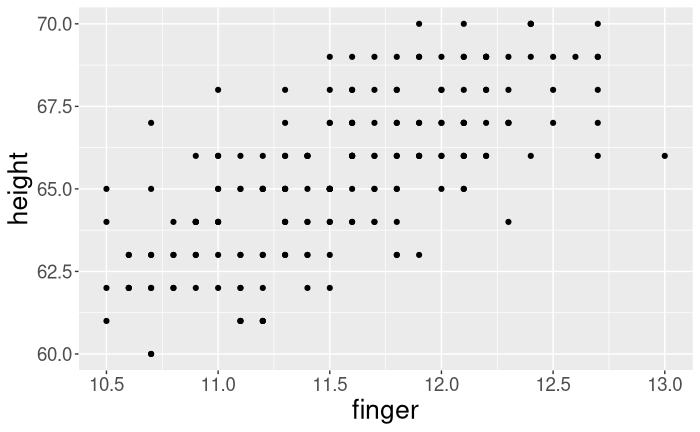
\includegraphics[scale = 0.4]{example1_SRS.png}
%  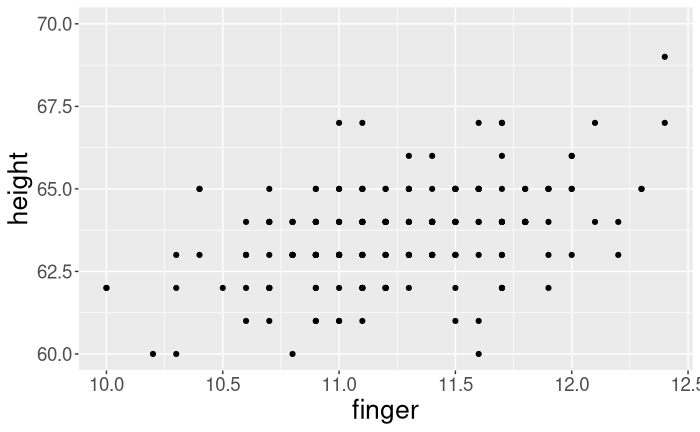
\includegraphics[scale = 0.4]{example1_UNEQ.png}
%  \caption{Two samples of finger length versus height. Left: Every person has the same
%    probability of being included in the sample. Right: The probability of being
%  included in the sample depends on height.}
%\end{figure}

The bottom row of figure \ref{fig:ex1} illustrate the difference between
classical regression and regression taking the probabilities of being included
in the sample into account. The bottom left plot shows regressions based on a
sample where every person has the same probability of being included. We can see
only one regression line is this plot, this is because both regression lines are
exactly equal in this case. In the bottom right plot of figure \ref{fig:ex1} we
see there are two different lines, the red one is the regression line from
classical regression while the blue line is from regression taking probabilities
for being included in the sample into account. The shaded areas represent 95\%
prediction intervals. We can see that the red line seems to fit the sample much
better than the blue one. The blue line seems too steep. This is because the
blue line takes into account the fact that the reason there are so few samples
in the top right of the plot is the fact that the people with long fingers had a
smaller chance of being included in the sample. When we look at the prediction
intervals we can see that the blue prediction interval seems to be ``correct''
by the metric that about 95\% of the dots are inside it, but the red one is far
from having that many dots.

These differences show that it is very important taking the design of the survey
into account when analyzing the data.

% The bottom row of figure \ref{fig:ex1} shows the difference between taking into account the
% sampling probabilities or not.
% In the top plots, where the regression lines are plotted on top of the unequal
% probability sample we can see that the line from normal linear regression, which
% is the red line, fits very well with the sample. While the line from linear
% regression taking into account the unequal sampling probabilities, the blue line, seems to be a
% bit too steep.

% When we look at the bottom plots however which show the regression lines on top
% of a sample where every one has equal sampling probabilities however we see that
% the line using normal linear regression, red line, is way too flat, while the
% one taking into account the sampling probabilities fits much better.
% By looking at the dashed lines which is a 95\% prediction interval we see that
% the prediction interval from the normal linear regression does not seem to
% include 95\% of the observations, while the one from the linear regression
% taking into account the sampling probabilities does.
\end{example}

The rest of the thesis focus's on a dataset on the performance of students in schools in
California. The dataset has data on all 6194 schools having more than 100
students in California, with data collected
including: API scores in 1999 and 2000, which level of school it is
(elementary, middle, high), name of school, location of school, percentage of
students tested at the school, API targets, economic factors for students at the
school, class sizes, information of education of parents and qualification of teachers.
API scores is a metric testing the academic performance of the students at the school.
We will use this data as the population we will sample from, and we will take
different kinds of samples to illustrate the concepts introduces in this thesis.

Section \ref{sec:modLinReg} will give a overview of model based simple
linear regression, this is assumed known and only a brief repetition will be given.
Section 3 will explain how to do linear regression in the context of finite
population using survey statistics. Section 3.1 will show how to do linear
regression when we have a Simple Random Sample. Section 3.2 will go through
linear regression when we have sample using stratification. Section 3.3 will
explain linear regression when having a sample using clustering and Section 3.4
will show how to do linear regression when you have surveys combining
stratification and clustering into a complex survey.


%The thesis will start by giving an introduction to survey statistics, where giving the necessary background theory needed to be able to talk about linear regression in this context.

\section{Classical simple linear regression} \label{sec:modLinReg}

TODO: Teksten er veldig to-the-point, noe jeg liker, men det kan bli litt intenst å lese for noen som ikke er kjent med survey statistics fra tidligere. Jeg tror noen enkle figurer vil hjelpe. Jeg tenkte at en enkel figur i Section 2 når du snakker om avstandene fra regresjonslinjen kunne vært fint også.

In classical simple linear regression, each observation \(i\) consists of a
response variable, \(y_i\), and a predictor, \(x_i\) for \(i = 1, ..., n\), where \(n\) is the number of observations. The
relationship between the response and the covariates is assumed to be
\begin{equation*}
Y_i = \beta_0 + \beta_1 x_i + \epsilon_i,\ i = 1, \dots, n,
\end{equation*}
where \(\epsilon_1, \epsilon_2, \dots, \epsilon_n\) are stochastic variables
describing the error and the intercept, \(\beta_0\), and the slope ,\(\beta_1\),
are constants that describe the deterministic part of this relationship.
We do not know the values of \(\beta_0\) and \(\beta_1\), so we have to estimate
them from observed data points.

We call these data points \((x_1, y_1), (x_2, y_2)
... (x_n, y_n)\). To estimate the deterministic part of the relationship we want
to find estimators \(\hat{\beta}_0\) and \(\hat{\beta}_1\) that minimize the
Residual Sum of Squared (RSS). The RSS is defined by
\begin{align*}
  \mathrm{RSS} &= \frac{1}{n} \sum_{i = 1}^n \left( y_i - \hat{y}_i \right)^2 
  = \frac{1}{n} \sum_{i = 1}^n \left( y_i - \hat{\beta}_0 - \hat{\beta}_1 x_i \right)^2.
\end{align*}
RSS can be geometrically thought of as the sum of the squared distances of
the data points in the sample from the regression line. Our goal is to find a
line that is as close as possible to the observed sample, and minimizing the RSS
is therefore one way to find a close line.

The estimators \(\hat{\beta}_0\) and \(\hat{\beta}_1\) that minimizes the RSS are
%$$
%\hat{\beta}_1 = \frac{\sum_{i = 1}^n\left( x_i - \bar{x} \right) \left( y_i -
    %\bar{y} \right)} {\sum_{i = 1}^n \left( x_i - \bar{x} \right)}
%$$
%and
%$$
%\hat{\beta}_0 = \bar{y} - \hat{\beta}_1 \bar{x}
%$$

\begin{equation*}
 \hat{\beta}_1 = \frac{\sum_{i = 1}^n\left( x_i - \bar{x} \right) Y_i}{\sum_{i = 1}^n\left( x_i - \bar{x} \right)^2} ,
\end{equation*}

\begin{equation*}
 \hat{\beta}_0 = \bar{Y} - \hat{\beta_1}\bar{x},
\end{equation*}
where \(\bar{x} = \frac{1}{n} \sum_{i = 1}^n x_i\) and \(\bar{y} = \frac{1}{n} \sum_{i = 1}^n y_i\).

Under the following conditions:

\begin{enumerate}
\item \(\mathrm{E} \left( \epsilon_i \right) = 0\ \forall \ i = 1, 2, ..., n\)
\item \(\mathrm{Var} \left( \epsilon_i \right) = \sigma^2\ \forall \ i = 1, 2, ..., n\)
\item All the \(\epsilon\) are independent of any predictor or observation number.
\item All \(\epsilon_1\), \(\epsilon_2\), ..., \(\epsilon_n\) are independent of each other.
\end{enumerate}

TODO: I Section 2 I teksten som følger etter de fire ligningene øverst på side 6, må du være mer korrekt. Du skriver “… as likely to be over the line as under it”. Dette er ikke riktig med mindre fordelingen til residualene er symmetrisk. Du burde skrive “… on average lie on the line” eller noe sånt. På samme måte må du være mer presis med utsagnet om item 2.


Item 1 means that data points should on average lie on the line.
TODO: Se over, spesiel
Item 2 means that the data points should have roughly the same vertical
Euclidean distance from the regression line.
Item 3 and 4 means that there should be no pattern in whether the data points is over
or under the regression line and on the vertical Eudlidean distance from the
regression line.

we get some useful properties, among which are these unbiased estimates for the
variance of the estimators \(\hat{\beta}_0\) and \(\hat{\beta}_1\)
\begin{equation*}
 \widehat{\mathrm{Var}} \left( \hat{\beta}_0 \right) = \frac{1}{n - 2} \sum_{i = 1}^n\left( y_i - \hat{\beta}_0 -
 \hat{\beta}_1 x_i \right)^2 \frac{\sum_{i = 1}^n x_i^2}{n
   \sum_{i = 1}^n \left( x_i - \bar{x} \right)^2}
\end{equation*}
 

\begin{equation*}
 \widehat{\mathrm{Var}} \left( \hat{\beta}_1 \right) = \frac{1}{n - 2} \sum_{i = 1}^n\left( y_i - \hat{\beta}_0 -
 \hat{\beta}_1 x_i \right)^2\frac{1}{
   \sum_{i = 1}^n \left( x_i - \bar{x} \right)^2},
\end{equation*}

where \(\frac{1}{n - 2} \sum_{i = 1}^n\left( y_i - \hat{\beta}_0 -
 \hat{\beta}_1 x_i \right)^2\) is an
unbiased estimator for the unknown \(\sigma^2\).

New: This is based on the fact that we assume the response is random, i.e, that
it is possible to get a different response if we measure again. This means we
can think of the residuals as coming from some stochastic distribution. What
happens, then, if we instead assume that the responses are fixed and are the
same if we measure them again?

This is the idea that survey statistics is based on.

Old: This is all based on the fact that the response has a distribution, which again
is based on the assumption that we have an infinite population to sample from.
What happens then, if we have a finite population? And what if the elements in
the sample are not independent of each other?

This is what survey statistics tells us.

TODO: skriv om, skriv på mer formell måte
The randomness does not arise from measurement but from selection


\section{Regression in the context of finite populations}
Now consider the case where the population is finite, i.e, the population
consists of \((x_1, y_1),
(x_2, y_2), \dots , (x_N, y_N)\), where the \(x_i\)'s are the covariates we use to
predict \(y_i\) and \(N\) is the size of the population.

The goal of linear regression in this case is that we want to find the linear
line, \(y = B_0 + B_1x\), that best describes the relationship between \(x_i\)
and \(y_i\) in this population. We define the best line as the one
that minimizes \(\mathrm{RSS} = \sum_{i = 1}^N (y_i - B_0 - B_1 x_i)^2\).
Minimizing the RSS means that we minimize the the squared Euclidian distance of each point
in the population from the line.

This differs from model based linear regression where we want to estimate the
deterministic part of the relationship between \(x_i\) and \(y_i\), but we can
never get an exact answer as the estimates will differ when they are based on
different samples, no matter how large. Here, however, we can find \(B_0\) and
\(B_1\), since we can sample the whole population if we want.

TODO:  Ligningen til slutt på side 6 kommer litt plutselig. Det hadde vært fint med litt mer forklaring.


If we know the whole population we can just compute \(B_0\) and \(B_1\) using the same formulas
as in Section \ref{sec:modLinReg}, which after rewriting them become
\begin{equation*}
 B_0 = \frac{1}{N} \left( t_y - \frac{t_{xy} t_x - \frac{1}{N} t_y t_x^2}
   {t_{x^2} - \frac{1}{N} t_x^2},
  \right)
\end{equation*}

\begin{equation*}
 B_1 = \frac{t_{xy} - \frac{1}{N} t_y t_x}
   {t_{x^2} - \frac{1}{N} t_x^2},
\end{equation*}
where \(t_x = \sum_{i = 1}^N x_i\), \(t_y = \sum_{i = 1}^N y_i, t_{x^2} =
\sum_{i = 1}^N x_i^2\) and \(t_{xy} =
\sum_{i = 1}^N x_i y_i\).

The case where we know the whole population is not realistic, we are instead interested in the case where we have to sample from the
population to estimate \(B_0\) and \(B_1\). To do that we have to introduce some terms:

TODO: I Definition 3.1 føler jeg sampling population versus sampling frame blir forvirrende. Kanskje det er bedre å forklare sampling frame I en separat definisjon.


\begin{definition} \label{def:sampUnitPopFrame}
 A \textbf{sampling unit} is one "element" we want to sample.
 The \textbf{sampling population}, or universe, \(U = \{1, 2, 3, ..., N\}\), is a
 finite set containing all the sampling units you are interested in. 
 The \textbf{sampling frame} is the list of all sampling units you are going to sample from. 
\end{definition}

In the case of our API dataset, our sampling units are schools, while
the sampling population is all the schools in California having more than 100 students.
The sampling frame would be all schools in California that the researchers know
about and that the researchers think have more the 100 students.
Ideally the sampling frame and the sampling population would be the same, but that is not always to case.
When taking different types of samples from the API dataset, the sampling population and the sampling frame are equal, since
we have a table of all the data and we will just choose rows from that table for
our samples. But there are cases where this is not the case. An example of this
could be if we were doing a political survey to try to predict who will win the
next election.
In that case our sampling population, who we are interested in information
about, would be everyone who are going to vote in the next election. It is
is impossible to get a list of them though, so we instead have to use 
some other part of the population we have information about. We might have a
list of all who voted last election, which might be a good approximation of
those who are going to vote this election, but then we would miss out on all the
new eligible voters and people who might have decided to vote this election but
didn't do it the last one.
Choosing the correct sampling frame to match your target sampling population is
difficult and getting it wrong will influence your results.

We will represent the sampling units by listing them in an arbitrary order and
then letting their indeces represent them. This simplifies notation.


\begin{definition} \label{def:sample}
A \textbf{sample}, \(S \subseteq U\), is a subset of the sampling frame. This is the data we will analyse to learn about the sampling population.
A \textbf{probability sample} is a sample where the sampling units included are chosen randomly.
The \textbf{sampling probability} of a sampling unit is the probability that a
specific sampling unit will be included in the sample.
\end{definition}


If we then let \(\hat{t}_x, \hat{t}_y, \hat{t}_{x^2}, \hat{t}_{xy}, \hat{N}\) be estimators
for \(t_x, t_y, t_{x^2},
t_{xy}, N\) respectively, we get the estimators for \(B_0\) and \(B_1\)
\begin{equation*}
 \hat{B}_1 = \frac{\hat{t}_{xy} - \frac{1}{\widehat{N}} \hat{t}_y \hat{t}_x}
   {\hat{t}_{x^2} - \frac{1}{\widehat{N}} \hat{t}_x^2}
\end{equation*}

\begin{equation*}
 \hat{B}_0 = \frac{1}{\widehat{N}} \left( \hat{t}_y - \frac{\hat{t}_{xy} \hat{t}_x - \frac{1}{\widehat{N}} \hat{t}_y \hat{t}_x^2}
   {\hat{t}_{x^2} - \frac{1}{\widehat{N}} \hat{t}_x^2}
 \right)
 = \frac{\hat{t}_y}{\hat{N}} - \hat{B}_1\frac{\hat{t}_x}{\hat{N}}
\end{equation*}

Since \(\hat{B}_0\) and \(\hat{B}_1\) are non linear expressions of dependent
statistics, deriving exact expressions for the variances can get very complicated. We, therefore,
often have to settle with having estimates of the variances instead.
There are several ways to do so, but a common one,
and the one we use in this thesis, is linearization. Linearization takes a
non-linear expression of stochastic variables we want to do inference about and uses
the first two terms of the Taylor expansion to make it linear.
For example, we have \(h(a, b, c, d, e) = \frac{ea - bc}{ed - b^2}\), such that
\(h(\hat{t_{xy}}, \hat{t_x}, \hat{t}_y, \hat{t}_{x^2}, \hat{N}) = \hat{B_1}\).
We then get
\begin{align*}
 \mathrm{Var}(\hat{B_1})
 &= \mathrm{Var} \left( h(\hat{t_{xy}}, \hat{t_x},
 \hat{t}_y, \hat{t}_{x^2}, \hat{N})) \right) \\
 &\approx \frac{\widehat{\mathrm{Var}}\left( \sum_{i \in S} w_i q_i \right)}
   {\left( \sum_{i \in S} w_i x_i^2 - \frac{\left( \sum_{i \in S} w_i x_i \right)^2}{\sum_{i \in S} w_i} \right)^2}
\end{align*}

where \(q_i = (y_i - \hat{B}_0 - \hat{B}_1 x_i)(x_i - \hat{\bar{x}})\).

TODO: Si noe om se seksjon 8 for fler detaljer om ikke-lineære uttrykk

\subsection{Simple random sample} \label{sec:SRS}

The simplest probability sample is the Simple Random Sample (SRS). A
sample of size \(M \leq N\) is an SRS if every subset \(S \subseteq U\) has the same
probability of being chosen.
If, for example, \(U = \{1, 2, 3, 4\}\) and we want a sample \(S\) of
size \(3\), then there are \(\binom{4}{3} = 4\)  possible samples:
%\begin{equation*}
%S_1 = \{1, 2, 3\}, 
%S_2 = \{1, 2, 4\}, 
%S_3 = \{1, 3, 4\}, 
%S_4 = \{2, 3, 4\} .
%\end{equation*}
\( S_1 = \{1, 2, 3\},\ \)
\( S_2 = \{1, 2, 4\},\ \)
\( S_3 = \{1, 3, 4\}\ \) and
\( S_4 = \{2, 3, 4\} \).

For this to be a SRS each of these subsets need to have the same probability of
being chosen, i.e, \(P(S_1) = P(S_2) = P(S_3) = P(S_4) = 0.25\). A consequence of
having a SRS is that all the sampling probabilities are equal, \(P(1 \in S) =
P(2 \in S) = P(3 \in S) = P(4 \in S) = 0.75\). But having equal sampling
probabilities is not sufficient for the sample to be an SRS.
Look, for example, at this case:
Assume we want a sample of size \(2\) from a population of size \(4\), and that
\(P(\{1, 3\}) = 0.5\) and \(P(\{2, 4\}) = 0.5\) while the probabilities of all the
other possible samples are \(0\). Then \(P(1 \in S) = P(2 \in S) = P(3 \in S) = P(4 \in S) = 0.5\)
but this is not a SRS since all possible subsets of size \(2\) do not have equal
probability of being chosen.


\subsubsection{Estimating regression coefficients}

We need estimates of several different totals of the population to estimate the
regression coefficients. We need the total of, among others, the \(y_i\)'s, the
\(x_i\) and the \(x_i * y_i\)'s, to calculate the estimates.
We will do inference on the total of the \(y_i\)'s here, but the other totals
are equivalent.

Let
\(
 t_y = \sum_{i = 1}^{N} y_i
\)
be the value we want to estimate.
The natural estimator of this total, if we sample \(n\) elements, would be
\(
\hat{t}_y = \frac{N}{n}\sum_{i \in S} y_i
\)
where we take the average of the values in our sample and then scale it up to
the whole population.
It can be shown using indicator variables and sampling probabilities that
\(\hat{t}_y\) is an unbiased estimator for \(t_y\).

\begin{definition}
 The \textbf{weight} of a sampling unit is the inverse of the sampling
 probability of the sampling unit. 
 We denote the weight of \(y_i\) as \(w_i\).
\end{definition}

TODO: Si mer om vekter, ta opp igjen diskusjonen i introduksjonen, hvor mange
datapunktet hver verdi svarer til. Hvorfor weight et intuitivt navn.

It can be shown that the sampling probability of a sampling unit in a SRS is
\(\frac{n}{N}\). This means that the weight of each sampling unit is
\(\frac{N}{n}\). We can therefore rewrite the estimator for \(t_y\) as
\(
\hat{t}_y = \sum_{i \in S} w_i y_i
\)

This is a convenient way to calculate estimates for more complicated sampling
schemes.

It can also be shown that the variance of the estimator is of the form \begin{equation*}
\mathrm{Var} \left( \hat{t}_y \right) = \frac{N^2}{n \left( N - 1 \right)} \left( 1 - \frac{n}{N} \right) \sum_{i = 1}^N (y_i - \bar{y})^2 
\end{equation*}

TODO: Mer forklaring.

where
\(
\frac{1}{N - 1} \sum_{i = 1}^N (y_i - \bar{y})^2
\)
is the variance of the whole population.
We do not, however, know the population variance, as that would require us to know the \(y\) values
for the whole population \(U\). Instead we estimate the population variance by the unbiased estimator\(
 \frac{1}{n - 1} \sum_{i \in S} \left( y_i - \hat{\bar{y}} \right)^2
\)
, where \(\hat{\bar{y}} = \frac{1}{n} \sum_{i \in S} y_i \), which gives us the estimate of \(\mathrm{Var}(\bar{y}_U)\)\begin{align*}
 \widehat{\mathrm{Var}(\hat{t}_y)}
 &=\frac{N^2}{\left( n - 1 \right)n} \left( 1 - \frac{n}{N} \right) \sum_{i \in S} \left( y_i - \hat{\bar{y}} \right)^2
\end{align*}
Since \(\frac{1}{n - 1} \sum_{i \in S} \left( y_i - \hat{\bar{y}} \right)^2\) is unbiased, we have that \(\widehat{\mathrm{Var}(\hat{t}_y)}\) is an unbiased estimator of the variance of \(\hat{t}_y\).

We see that all these estimators for totals and means are the same as in the
model based case. Therefore the estimates for the coefficients in the regression
model are also the same. The variance of the estimators for the coefficients are
different however.
The factor \(\left( 1 - \frac{n}{N} \right)\) in the variances is what differs in
the variance estimate compared to the model based one. It is called the
\textbf{finite population coefficient (fpc)} and comes from the fact that we are
sampling without replacement from a finite population.
When we sample a larger and larger portion on the population we will get more
and more information and therefore the variance will decrease towards zero.
This means that if the population size decreases but the sample size stays the
same the variance will decrease, as there are fewer unmeasured sampling units.

Using linearization we get this estimate for the variance of \(\hat{B}_1\) when
the sample is from an SRS\begin{equation*}
\widehat{\mathrm{Var}}(\hat{B}_1) = \left( 1 - \frac{n}{N} \right) \frac{n}{n - 1} \frac{\sum_{i \in S} \left( x_i - \bar{x} \right)^2 \left( y_i - \hat{B}_0 - \hat{B}_1 x_i \right)^2}
{\left( \sum_{i \in S} \left( x_i - \bar{x} \right)^2 \right)^2}
\end{equation*}

which we can compare to the estimate of the variance for \(\hat{\beta}_1\) in
the model based case
\begin{equation*}
 \widehat{\mathrm{Var}} \left( \hat{\beta}_1 \right) = \frac{\sum_{i = 1}^n\left( y_i - \hat{\beta}_0 -
 \hat{\beta}_1 x_i \right)^2}{
   \left( n - 2 \right)\sum_{i = 1}^n \left( x_i - \bar{x} \right)^2}.
\end{equation*}


\subsection{Stratification} \label{sec:strat}

In stratification we split the sampling frame into a partition, i.e, \(H\) non
overlapping subsets that together comprise the whole sampling frame. These
subsets are called \textbf{strata}. We let each stratum have \(N_i,\ i = 1, \dots
, H,\) elements, and \(N_1 + N_2 + \dots + N_H = N\). When sampling we
indepentently take samples from each stratum, \(S_1, S_2, \dots, S_H\), with \(n_i,\ i = 1, \dots
, H,\) elements. When
estimating a total we can therefore first estimate the total of each stratum and
then add these totals to get an estimate of the population total.
If we let \(t_{y,h}\) be the total in stratum \(h\) we get \(\hat{t}_y =
\sum_{h = 1}^H \hat{t}_{y, h} \), where we can use different sampling schemes to
estimate each \(t_{y, h}\).
If we let each sample of the subsets be a simple SRS we get \( \hat{t}_y =
\sum_{h = 1}^H\sum_{i \in S_h}\frac{N_h}{n_h}y_i = \sum_{i \in S} w_i y_i\),
where \(S = S_1 \cup S_2 \cup \dots \cup S_H\).
Since the estimate for each
stratum total is unbiased, see section \ref{sec:SRS}, the estimate of the population
total is unbiased.

% TODO: skriv hva w_i er. Vekter estimater fra hvert stratum forskjellig. Hvor mye
% hver observasjon teller.
% Legg til eksempel. To strata med forskjellig forventningsverdi. Se på bias med
% forskjellig sample størrelse.

Since we often sample differently in the different strata,
the individuals sampled from the different stratum usually have
different sampling probabilities. This means that the sampling weights also
differ as they are the inverse of the sampling probabilities.

\begin{example}
  Suppose a population is divided into two strata, each with a population of
  \(1000\) individuals. Let one be values from a normal distribution with mean
  \(0\) and variance \(1\) and one with mean \(10\) and variance \(1\), called
  \(A\) and \(B\).
  \textbf{Dumt å si at de er fra en fordeling?}.
  Our goal is to estimate the sum of the values.

  The true sum of the population values is \(10058.59\). If we sample the same
  proportion of values from \(A\) and \(B\) we can estimate the sum the same way
  as in a SRS. Let \(S_{A, 100}\) and
  \(S_{B, 100}\) be SRS's of size \(100\) from \(A\) and \(B\) respectively.
  Then an unbiased estimate of the total is \(\sum_{i \in S_{A, 100} \cup S_{B,
      100} } \frac{2000}{200} y_i = 10104.81\). The bias is only \(46.22\) which is only \(0.46\%\) of the
  value.

  If we sample different proportions of values from \(A\) and \(B\), however, we
  can't use this simple estimate. Let \(S_{A, 50}\) be a SRS of size \(50\)
  from \(A\). If we use the same SRS estimate again we get \(\sum_{i \in S_{A, 50} \cup S_{B,
      100}} \frac{2000}{150} y_i = 13560.02\). The bias is here \(3501.425\) which is \(34.8\%\) of the
  value. This is a much larger error. This is because we have more samples from
  \(B\) than \(A\), and \(B\) has a higher mean than \(A\). Since each sampled
  value is counted the same this causes the estimate to become too large. To fix
  this we need to let the sampled values from \(A\) count, or weigh, more than
  the ones from \(B\). This is because the values in \(S_{A, 50}\) have to
  represent the same size population as the values in \(S_{B, 100}\), but there
  are only half as many values in \(S_{A, 50}\) as in \(S_{B, 100}\). Therefore,
  each value in \(S_{A, 50}\) has to count two times as much as the values in \(S_{B, 100}\).

  Doing this the estimate becomes \(\sum_{i
    \in S_{A, 50}} \frac{1000}{50} y_i + \sum_{i \in S_{B, 100}}
  \frac{1000}{100} = 10174.61\) which has a bias of \(116\) which is \(1.15\%\),
  a huge improvement over the \(34.8\%\) bias where we did not take the
  different sampling probabilities into account.
\end{example}

TODO: kan gjenta introduksjonen når det gjelder vekter.

This illustrates the importance of using the correct weights. In the example the
values in \(S_{A, 50}\) had a lower sampling probability than the ones in
\(S_{B, 100}\), which means that their weights increase, since they are the
inverse of the sampling probability.

Since the samples from the different strate are independent the variance of the estimator is also
easy to calculate: \(\mathrm{Var}(\hat{t}) = \mathrm{Var}\left(\sum_{h =
   1}^H\sum_{i \in S_h}\frac{N_h}{n_h}y_i\right) = \sum_{h =
   1}^H\mathrm{Var}\left(\hat{t}_{y, h}\right)\). This
means that to minimize the variance of \(\hat{t}\) we should choose the strata
such that the internal variance is as small as possible.

Stratification is used for several reasons; making it possible to analyze
subpopulations individually, making sure subgroups are included in the sample
and reducing uncertainty.

If we have a population with several different interesting subgroups it can be
useful to let each of these subgroups be their own strata. This will allow us to
create seperate regression lines for each strata, which will allow us to
analyze them by themselves. We can then compare the slopes to see if there is a difference in the relationship between the
response and predictor for the different strata. We could of course make
regression lines for different subgroups after doing a sample without strata,
but then we would have no guarantee that each of the subgroups would have enough
samples to be able to make a useful regression line. Using stratification we can
choose how many samples we want from each subgroup.

% Suppose we want to sample schools in the API dataset to learn about the student
% performance throught the API metric. We might reasonably assume that students
% having parents with higher education will get more help at home for schoolwork
% and therefore perform better in school. It might therefore be reasonable to
% create strate that splits the population by the percentage of parents with a
% college degree. If we take an SRS of size \(300\) of all the schools we get an API mean of
% \(659.37\) with a variance \(56.36\). However if we take a stratified sample,
% where the strate are the schools with less than \(20\%\) of parents having
% college degrees, schools with between \(20\%\) and \(40\%\) of parents having
% college degrees and schools with more than \(40\%\) of parents with college
% degrees, and we take a sample of 100 schools from each stratum, we get an API
% mean of \(668.33\) and variance \(43.37\). Since we have the full dataset we can
% find the true mean, which is \(664.7\), so both methods were roughtly the same
% distance from the correct value. However the variance from the stratified sample
% is smaller. In addition we have the option of finding the mean of each of the
% strata separately without taking new samples.

TODO: Velger ofte ikke sample størrelse etter populasjonsstørrelse, velger
heller en absolutt størrelse.

\begin{example}
  Suppose that we want to investigate the relationship between the API score of
  a school and the average level of education of the student's parents. We might
  be interested in knowing if the effect the parents education level has on
  their childs performance changes as they get older. It would therefore make
  sense to stratify on which level the school is, elementary school, middle
  school or high school. We can then see if the estimated slope coefficient is
  different in each of these strata.
  The population has \(4421\) elementary schools, \(755\) middle schools and
  \(1018\) high schools and we choose to sample \(50\) schools from each strata.

  The table shows the estimated slope for each school level. We can see that
  parent education level seems to have a higher effect in Elementary schools
  than higher school levels. Regression on all the strata together gives the
  slope \(158\), which is somewhere in between all the individual slopes. Not
  doing stratification would therefore make us loose the information for each
  school type.

  TODO: Ta med sanne verdier. Lag konfidensintervall.

  \begin{center}
  \begin{tabular}{ccc}
    %\label{table:stratExCoef}
    %\caption{Test}
    Elementary schools & Middle schools & High schools \\
    \hline \\
    169.1 & 145 & 143.8
  \end{tabular}
  \end{center}
\end{example}


\subsection{Clustering}


In clustering we split the sampling frame into a partition as in stratification.
Here, however, we do a probability sample to choose which of the subsets we will
collect data from, which is now \(S\). Then we have to do a probability sample
inside of each of these chosen subsets, \(S_1, S_2, \dots, S_n\).

\begin{definition}
 \textbf{Primary sampling unit (psu)} are subsets of the sampling frame, that
 are sampled first in a sampling scheme. TODO: Kalles ofte cluster, men bare psu. \\
 \textbf{Secondary sampling unit (ssu)} are smaller subsets of the sampling
 frame, each included in ppus. The ssus are often individual units in the
 sampling frame. TODO: Ta ssu i teksten, brukes i multistage clustering.
\end{definition}

There are two ``types'' of cluster sampling; one-stage cluster sampling and
multi-stage cluster sampling. In one-stage cluster sampling we sample all the
elements in the subsets chosen in \(S\), so each element has probability \(1\)
of being included. In multi-stage cluster sampling, however,
we make a sample of the ssus inside the psus in \(S\), where not all ssus are
included in the sample. Multi-stage cluster sampling is often what is used in
practice, but since the idea is so similar and the formulas get so complicated
we will restrict outselves to one-stage cluster sampling in this thesis.

the ppus are the subsets from the
partitioning and the ssus are the individual sampling units.

Let \(N\) be the number of clusters (psus) in the population and let \(M_i,\ i =
1, 2, \dots, N\) be the number of individuals (ssus) in each cluster. Let
\(t_{y, i}\) be the total for cluster \(i\), Since we know the totals for the
clusters in the sample \(S\), we can consider each cluster a sampling unit as we
have done earlier in the thesis. In one-stage cluster sampling, an SRS is
usually taken to choose which clusters to include in the sample. This gives the
same estimator for the total as for a SRS, except that the sampling units here
are the totals for each cluster instead of individuals as in a normal SRS,
\(\hat{t}_y = \sum_{i \in S} \frac{N}{n} t_{y, i} = \sum_{i \in S} w_i t_{y, i} \). 
This also gives the same estimate for the variance as in an SRS,
\(\widehat{\mathrm{Var}}\left(t_{y}\right) = \frac{N^2}{n} \left( 1 - \frac{n}{N}
\right) \hat{\mathrm{Var}}\left( t_{y, i} \right) =
\frac{N^2}{\left( n - 1 \right)n} \left( 1 - \frac{n}{N} \right) \sum_{i \in S}
\left( t_{y, i} - \hat{\bar{t_y}} \right)^2\), where \(\hat{\bar{t_y}} =
\frac{1}{n} \sum_{i \in S} t_{y, i}\).

Larger populations often mean that the totals for that population is also large,
for example when we are measuring API scores for schools, the total of all the
schools in a population will increase as the number of schools we sample
increase, as the score is always positive. This means that the variance of the
total estimates will usually increase if the clusters have very different
population sizes. It can therefore be useful to try to keep the populations in
the different clusters as similar as possible. But one should be careful not
putting too much weight on keeping the population sizes equal, as that may cause
the clusters to become too spread out physically which will make it expensive to
measure all individuals in it, which will again defeat the purpose of clustering
in the first place.

This means that a cluster sample with the same number of individuals in it will
almost always have a larger variance than a SRS of the same size. This is
becuase individuals inside a cluster will usually be more similar than
individuals across clusters. This means that measuring say \(10\) people inside
one cluster will give less information than measuing \(10\) people randomly
chosen in the whole population, which will cause a larger uncertainty. Measuring
inside a cluster is often cheaper than measuring people sampled randomly from
the whole population though. For example if the clusters are geographical areas,
which they usually are and each individual sampled needs a researcher or
interviewer to physically show up, then one will save a lot of time and money
not having to travel to so many different places. This means that it is often possible to sample
many more individuals in cluster sampling than when doing samples from the whole
population, which will decrease the uncertainty and make cluster sampling more
competitive with other sampling methods.

\begin{example}
  We again look at the API dataset. Let us suppose that to collect the data, an
  interviewer has to travel to each school. Then it would take a lot of time and
  get very expensive if they had to travel to random schools all over
  California. It would then be a lot cheaper and take a lot less time to just
  collect data in some chosen school districts, we therefore choose to cluster
  on them. There are \(757\) school districts in California and we take a SRS to
  get a sample of \(15\). This gives us a sample of \(183\) schools.
  %Figure \ref{fig:exClus} shows how the prediction interval of the regression line
  %based on the clustered sample is larger than the prediction interval of a SRS
  %of size \(183\).

  \begin{figure}
    \centering
    \includegraphics[scale = 0.5]{exClus}

    \caption{Plot of regression line for a clustering sample. The red line is
      the regression line from analyzing the sample as a clustered sample. The
      blue line is the regression line from analyzing the clustered sample as an
    SRS. The shaded areas are the regression lines prediction intervals.}

    \label{fig:exClus}
  \end{figure}

  In Figure \ref{fig:exClus} we show regression lines from analyzing the sample
  in two ways. For the red line, we did it the ``correct'' way. We have taken
  the sampling scheme into account, so the correlation between the individuals
  in the same cluster is corrected for. For the blue line we ignored the
  clustering and analyzed the sample as if it was a SRS. This ignores all
  correlation between the individuals.
  TODO: Gi tall på hvor mange punkter er inni prediksjonsintervall

  We can see from the prediction intervals, the shaded areas, that clustering
  gives more uncertainty than a SRS of the same size. This makes sense, as each
  individual in the clustered sample carries a lot less information than each
  individual in an SRS, as the individuals inside a cluster can usually be
  assumed to be more similar the individuals in different clusters.

\end{example}

\subsection{Complex surveys}

TODO: Ta opp utviklingsland, vet ofte heller ikke populasjonen.
Trenger stratum for counties og urban vs rural
Må gjøre clustering for å unngå å reise rundt i hele Kenya.

In most surveys performed both stratification and clustering is used. One would
often, for example, first stratify on the different parts of the population you
are interested in, and then use clustering within each strata.

In practice we often combine clustering and stratification to what is called a
\textbf{complex survey}. 

\section{Variance estimation}

A central part of doing statistics is the calculation of uncertainties. We
usually express the uncertainty by estimating variance. Without an idea of the
variance of an estimated value, the estimate is all but useless, as the variance
could be so large that almost any confidence interval will include all possible
values. It is therefore very important to have a reasonable estimate of the
variance. The problem, however, is that in regression the values we are
interested in are non-linear expressions. We therefore can't find a closed form
expression for the variance estimate using normal rules, so we instead have to
use other techniques to
find variance estimates. One of the more used methods in survey
statistics, and one which will give a closed form expression for the estiamate,
is linearization.

TODO: Ha med eksempel med tall, enten i dette eksempelet eller lag et nytt.

\begin{example}
  TODO: Forklar stegene bedre, f.eks. hvorfor sentrere på sanne verdier.
  Let \(\widehat{W} = \frac{\hat{t}_y}{\hat{t}_x}\), where \(\hat{t}_y\) and \(\hat{t}_x\) are stochastic variables. We
  are interested in finding \(\mathrm{Var} \left( \widehat{W} \right) = \mathrm{Var}
  \left( \frac{\hat{t}_y}{\hat{t}_x} \right)\).
  Since this is a non-linear expression, there is no easy formula to calculate
  it. We do, however, know how to calculate the variance of a linear
  combination. We can therefore take advantage of the fact that we can
  approximate \(\widehat{W} = \frac{\hat{t}_y}{\hat{t}_x}\) by using a first degree Taylor approximation,
  which is linear.

  Let \(h(a, b) = \frac{a}{b}\). Then \(\widehat{W} = h(\hat{t}_y, \hat{t}_x)\).
  \(h'(a, b) = \begin{bmatrix} \frac{1}{b} & -\frac{a}{b^2} \end{bmatrix}.\)

  This means that
  \begin{align*}
    \widehat{W} &= h(\hat{t}_y, \hat{t}_x)
    \approx h(t_y, t_x) + h'(t_y, t_x) \left( \begin{bmatrix} \hat{t}_y \\ \hat{t}_x \end{bmatrix}
    - \begin{bmatrix} t_y \\ t_x \end{bmatrix} \right)
    = \frac{t_y}{t_x} + \begin{bmatrix} \frac{1}{t_x} &
    -\frac{t_y}{t_x^2} \end{bmatrix} \begin{bmatrix} \hat{t}_y - t_y \\
      \hat{t}_x - t_x \end{bmatrix} \\
    &= \frac{t_y}{t_x} + \frac{1}{t_x} \left( \hat{t}_y - t_y \right) - \frac{t_y}{t_x^2} \left( \hat{t}_x - t_x \right)
    \end{align*}

    Since \(t_y\) and \(t_x\) are deterministic values, they have zero variance
    and we can ignore them in the variance expression. We can therefore apply
    the standard rules for calculating variances of linear expressions and we
    get that
    \begin{align*}
      \mathrm{Var} \left( \widehat{W} \right) \approx \mathrm{Var} \left(
      \frac{t_y}{t_x} + \frac{1}{t_x} \left( \hat{t}_y - t_y \right) -
      \frac{t_y}{t_x^2} \left( \hat{t}_x - t_x \right) \right)
    = \frac{1}{t_x^2} \mathrm{Var} \left( \hat{t}_y \right) +
      \frac{t_y^2}{t_x^4} \mathrm{Var} \left( \hat{t}_x \right),
      \end{align*}
      which gives the simple expression \begin{align*}
                    \widehat{\mathrm{Var}} \left( \widehat{W} \right) = \frac{1}{\hat{t}_x^2} \widehat{\mathrm{Var}} \left( \hat{t}_y \right) +
                    \frac{\hat{t}_y^2}{\hat{t}_x^4} \widehat{\mathrm{Var}} \left( \hat{t}_x \right)
                    \end{align*}

    Since \(\hat{t}_y\) and \(\hat{t}_x\) are linear expressions we are able to
    find closed form expressions for their variance estimates and we can
    therefore calculate \(\widehat{\mathrm{Var}} \left( \widehat{W} \right)\).

\end{example}

More generally, let \(h(x)\), where \(x = (x_1, x_2, \dots, x_p)\), be a function such that \(h(x) = \theta\), where
\(\theta\) is the statistic we are interested in. Further, let \(\hat{x}\) be an
estimate of \(x\), such that \(h(\hat{x}) = \hat{\theta}\). If \(h\) is
linear, there is no problem finding a closed form for the variance estimate,
so we assume here that \(h\) is a non-linear function.

TODO: Se på grensene i integralet
By Taylor's theorem, we know that \(h(\hat{x}) = h(x) + h'(x) (\hat{x} - x) + \int_x^{\hat{x}}  (\hat{x} -
t) h''(t) dt\), where the last term is usually small compared to the first two
in statistics. This allows us to use the approximation \(h(\hat{x}) \approx h(x) +
h'(x) (\hat{x} - x)\). \(h(x) = \begin{bmatrix} \frac{\partial h}{\partial x_1}
  (x_1) & \frac{\partial h}{\partial x_2} (x_2) & \dots & \frac{\partial
    h}{\partial x_p} (x_p)\end{bmatrix}\), which means that \(h(\hat{x}) \approx
h(x) + h'(x) (\hat{x} -
x) = h(x) + \sum_{i = 1}^p \frac{\partial h}{\partial x_i} (x_i) \left( \hat{x}_i - x_i
\right)\), which is a linear expression in \(\hat{x}\). Using normal rules for
variance estimation of linear expression we have
\begin{align*}
  \mathrm{Var} \left( \hat{\theta} \right)
  &= \mathrm{Var} \left( h(\hat{x}) \right)
  \approx \mathrm{Var} \left( h(x) + \sum_{i = 1}^p \frac{\partial h}{\partial x_i} (x_i) \left( \hat{x}_i - x_i
    \right) \right) \\
    &= \sum_{i = 1}^p \left( \frac{\partial h}{\partial x_i} (x_i)  \right)^2 \mathrm{Var} \left( \hat{x}_i \right) + \sum_{i \neq j}  \frac{\partial h}{\partial x_i} (x_i)  \frac{\partial h}{\partial x_j} (x_j)  \mathrm{Cov} \left( \hat{x}_i, \hat{x}_j \right)
\end{align*}
We do not, however, know \(x\), as that are the true values we are trying to
estimate. But by replacing \(x\) by \(\hat{x}\), and by replacing the variances
of \(\hat{x}\) by estimated variances in the expression we get an
estimate of the variance
\begin{align*}
  \widehat{\mathrm{Var}} \left( \hat{\theta} \right)
  = \sum_{i = 1}^p \left( \frac{\partial h}{\partial x_i} (\hat{x}_i)  \right)^2 \widehat{\mathrm{Var}} \left( \hat{x}_i \right) + \sum_{i \neq j}  \frac{\partial h}{\partial x_i} (\hat{x}_i)  \frac{\partial h}{\partial x_j} (\hat{x}_j)  \widehat{\mathrm{Cov}} \left( \hat{x}_i, \hat{x}_j \right)
\end{align*}

In the regression case, the differentiation, and the estimates of covariance
gets pretty complicated, so we won't show the derivation here, but by using
similar techniques one can show that
\begin{align*}
 \mathrm{Var}(\hat{B_1})
 &= \mathrm{Var} \left( h(\hat{t_{xy}}, \hat{t_x},
 \hat{t}_y, \hat{t}_{x^2}, \hat{N})) \right) \\
 &\approx \frac{\widehat{\mathrm{Var}}\left( \sum_{i \in S} w_i q_i \right)}
   {\left( \sum_{i \in S} w_i x_i^2 - \frac{\left( \sum_{i \in S} w_i x_i \right)^2}{\sum_{i \in S} w_i} \right)^2}
\end{align*}
where \(q_i = (y_i - \hat{B}_0 - \hat{B}_1 x_i)(x_i - \hat{\bar{x}})\).

``Under conditions commonly satisfied in statistics, the last term is small
relative to the first two ...'' \textbf{Dette er et sitat fra boka, men de
  utdyper det ikke noe mer. Burde jeg finne en referanse på det?}


Linearisering
TODO: Eksempel, litt enkelt, bare en enkel brøk.

Hvorfor ting vanskelig.
Kan bruke linearisering.

Resampling hvis vi har tid

\section{Discussion}
Ta opp viktigste poenger.
Må gjøre varianskorreksjon.

har ikke trukket tilfeldig.

stratifisering

clustering
  Kan ikke gjøre dette i model based

blir vanskelig å diskutere varians

Veldig nyttig

Ingen formler.

Hvis du har gjort clustering og stratifisering er det direkte feil med model
based. Se eksempel 1. Survey statistics er alltid riktig, model based noen ganger.

Disse type metoder brukes ofte for å estimare dødelighet, vaksinasjonsrate og
lignende i utviklingsland. Mest i clustering, litt her i diskusjonen.
https://ntnuopen.ntnu.no/ntnu-xmlui/handle/11250/2624622 er master oppgave jeg
kan se på og referere til. Spesielt interessant er 1.3.
https://dhsprogram.com/pubs/pdf/fr308/fr308.pdf er rapport om Kenya som
masteroppgaven over bruker. Kan referere til den.

TODO: Du trenger en referanseliste til slutt og noen refereranser underveis. Spesielt i forbindelse med least squares estimatorene i Section 2, og noen av uttrykkene i Section 3. Det ville også vært fint å hatt en eller to referanser i Section 1.
Natbib: citations, navn og årstall (authoryear)

Cit seksjon 2, bok fra ST1101

\end{document}